\providecommand*{\lstnumberautorefname}{line}

High-level Synthesis tools, like LegUp or VivadoHLS, can automatically generate an FPGA 
circuit for the matrix multiplication example in Listing \ref{lst:MMM}.
What if the designer was required to run this circuit reliably in the
presence of soft errors? 
The naive approach would be to instantiate multiple copies of the circuit and run
them in lock-step on the same input data with any deviations between them
indicating an error.

\lstset{language=C}
\begin{lstlisting}[basicstyle=\ttfamily\footnotesize, frame=single, label={lst:MMM}, captionpos=b, caption={Matrix Multiplication Example},numbers=left,escapeinside={@}{@}]
void MMM(float A[5][5],float B[5][5],float C[5][5])
{ int i=0, j=0, k=0;
  for(i=0, i<5, i++){
    for(j=0, j<5; j++){
      C[i][j] = 0;
      for(k=0, k<5; k++){
        @\label{lst:MMM_2}@C[i][j] += A[i][k]*B[k][j]; }
    }
  }
}
\end{lstlisting}

Replication in this fashion is expensive in both area and more importantly
power, especially in this example as expensive floating point arithmetic
units are required for the calculation of the inner dot product.

\begin{figure}[h]
\centering
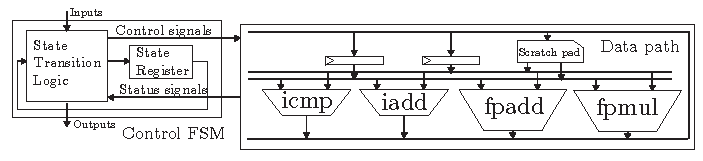
\includegraphics[width=3.5in]{./imgs/singleHLSArch_v2.pdf}
\caption{Diagram representing a HLS circuit for the Matrix Multiplication example}
\label{fig:singleHLSArch}
\end{figure}

If tight constraints prevent full replication then reliability can still be
improved through selectively replicating "important" portions of the design.
Various studies have shown that for a number of applications there exist critical regions
of code sensitive to soft errors and non-critical regions which are less sensitive.
This is especially true in applications involving media processing or machine
learning\cite{wong2006soft} \cite{liu2012flikker}.

%What about just the control flow?
Control-flow regions, (i.e. instructions effecting branch decisions), are arguably more critical
than data-flow, since faults within control-flow can effect real time guarantees
and termination.
Research into HLS for VLSI designs has proved promising for control-flow intensive
(CFI) applications \cite{chen2014reliability,chen2015reliability}, and fault injection
results have shown that control-flows are highly vulnerable to errors
\cite{saggese2005microprocessor, nakka2007processor, wong2006soft}.

%In our example what would control flow errors do?
Faults within the control structure for our matrix multiplication example
could cause the calculation of rows and columns of the output matrix \lstinline$C$ to be skipped,
or even worse, cause the circuit to enter an infinite loop and never terminate.
This paper presents an approach for automatically extracting the control flow structure
for a HLS application so that this region of the design can be selectively
replicated to protect control decisions.

Figure \ref{fig:singleHLSArch} provides a diagram of the HLS generated
circuit for our matrix multiplication example.
Two clear partitions can be seen, a data path where functional units reside, and a
control FSM responsible for scheduling instructions onto the functional units.
In order to replicate only the control-flow structure
any data-path functional units which may influence a state transition need to be
duplicated along with the control FSM.

Analysing the code in Listing \ref{lst:MMM} we can determine that the instructions
which influence control-flow decisions are the ones used in the \lstinline{for} loop
conditions, which require an integer comparator \textbf{icmp} and adder \textbf{iadd}.
While the expensive floating point units, \textbf{fpmul} and \textbf{fpadd}, required
for calculating the inner dot product on line 7 have no
influence over any branch decision and will not be replicated.

Manually inspecting code and removing elements that don't influence control flow
may be feasible in the simple case of Matrix Multiplication, however as the complexity of the input increases
the engineering effort required in both analysing the input source and a generating circuit with an identical control FSM is
significant.
StitchUp fully automates this process through using a static analysis technique, known as program slicing, to extract
and duplicate any instructions that may influence control. The contribution of this paper are:
\vspace{-4pt}
\begin{itemize}
	\setlength{\itemsep}{1pt}
	\setlength{\parskip}{0pt}
	\setlength{\parsep}{0pt}
	\item StitchUp, a tool which can automatically extract and protect the control flow structure of a circuit generated with a HLS tool.
	\item Detailed results of StitchUp on the CHStone benchmark, where exhaustive hardware fault injection is performed on the majority of cases.
	\item Results exploring the reliability of StitchUp protected circuits as the control to data ratio is varied through
	loop unrolling in the matrix multiplication example.
\end{itemize}

